%------------------------------------------------------------
\title[09 - 内存空间与指针]
{09 - 内存空间与指针}

\subtitle{C++ 程序设计进阶}

\author[Beiyu Li]
{Beiyu Li\\
\texttt{<sysulby@gmail.com>}}

% \institute[SOJ]
% {Sicily Online Judge}

\date[\today]
{\number\year 年 \number\month 月 \number\day 日}
%------------------------------------------------------------


\begin{document}

\author[sysulby]
{SOJ 信息学竞赛教练组}

\begin{frame}
    \titlepage
\end{frame}
\setcounter{framenumber}{0} % 标题页不编号

%------------------------------------------------------------
\begin{frame}[fragile]
    \frametitle{讨论}

    \begin{block}{}
        \vspace{.5cm}
        \begin{center}
            {\Large 为什么数组通常声明在函数外面?}
        \end{center}
        \vspace{.5cm}
    \end{block}
\end{frame}
%------------------------------------------------------------

\section{内存空间}

%------------------------------------------------------------
\begin{frame}[fragile]
    \frametitle{C++ 内存区域划分}

    \begin{table}[!ht]
        \centering
        \renewcommand{\arraystretch}{1.5} % 设置垂直内边距为1.5倍默认行高
        \begin{tabular}{cc}
            \toprule
            \textbf{区域}  & \textbf{用途} \\
            \midrule
            栈区(\lstinline|stack|)  & 存储局部变量、调用函数时需保存的信息 \\ 
            堆区(\lstinline|heap|)   & 用于动态内存分配 \\ 
            全局区、静态区(\lstinline|static|)   & 存放全局变量和静态变量 \\ 
            代码段(\lstinline|text|)  & 存放代码指令 \\
            \bottomrule
        \end{tabular} 
    \end{table}

\end{frame}
%------------------------------------------------------------

%------------------------------------------------------------
\begin{frame}[fragile]
    \frametitle{全局区、静态区(\lstinline|static|)}
    
    \begin{itemize}  
        \item 全局区,也称静态区,是用于存储全局变量和静态变量的一块内存区域
        \item 全局区由编译器在程序编译阶段分配,并且在程序运行期间始终存在,在程序结束后由系统释放
        \item 对于全局区的基本类型变量,声明时如果没有赋值,会被默认初始化为 0
    \end{itemize}

\end{frame}
%------------------------------------------------------------

%------------------------------------------------------------
\begin{frame}[fragile]
    \frametitle{栈区(\lstinline|stack|)}
    
    \begin{itemize}
        \item 栈区是由编译器自动管理的一种内存,用于储存函数的局部变量以及其他临时数据
        \begin{itemize}
            \item 声明局部变量 $a$ 时,$a$ 被储存在栈区中,$a$ 所在的代码块执行结束时,$a$ 所占用的内存会被自动释放
        \end{itemize}
        \item 栈区在存储、释放数据时,具有先存储的内容后释放的特点(先进后出)
    \end{itemize}

\end{frame}
%------------------------------------------------------------

%------------------------------------------------------------
\begin{frame}[fragile]
    \frametitle{示例:三个数的和}

    \begin{columns}
        \column{.70\textwidth}
        \lstinputlisting[basicstyle=\ttfamily\scriptsize,language=C++,name=sum3]{ch21/sum3.cc}
        \begin{tikzpicture}[remember picture,overlay]
            \uncover<1>{\redbox{sum3}{7}{1}{7}{12};}
            \uncover<2>{\redbox{sum3}{8}{1}{8}{14};}
            \uncover<3>{\redbox{sum3}{9}{1}{9}{21};}
            \uncover<4>{\redbox{sum3}{10}{1}{10}{32};}
            \uncover<5>{\redbox{sum3}{10}{1}{10}{32};   \redbox{sum3}{4}{1}{4}{31}; 
                \draw[red, very thick, ->] ([shift={(2pt, .25em)}] pic cs:line-sum3-10-end) -- ++(3em, 0) |- ([shift={(2pt, .25em)}] pic cs:line-sum3-4-end);}
            \uncover<6>{\redbox{sum3}{5}{1}{5}{24};}
            \uncover<7>{\redbox{sum3}{5}{1}{5}{24};    \redbox{sum3}{1}{1}{1}{24}; 
                \draw[red, very thick, ->] ([shift={(2pt, .25em)}] pic cs:line-sum3-5-end) -- ++(3em, 0) |- ([shift={(2pt, .25em)}] pic cs:line-sum3-1-end);}
            \uncover<8>{\redbox{sum3}{2}{1}{2}{15};}
            \uncover<9>{\redbox{sum3}{2}{1}{2}{15};   \redbox{sum3}{5}{1}{5}{24};
                \draw[red, very thick, ->] ([shift={(2pt, .25em)}] pic cs:line-sum3-2-end) -- ++(8em, 0) |- ([shift={(2pt, .25em)}] pic cs:line-sum3-5-end);}
            \uncover<10>{\redbox{sum3}{5}{1}{5}{24};  \redbox{sum3}{10}{1}{10}{32};
                \draw[red, very thick, ->] ([shift={(2pt, .25em)}] pic cs:line-sum3-5-end) -- ++(6em, 0) |- ([shift={(2pt, .25em)}] pic cs:line-sum3-10-end);}
        \end{tikzpicture}

        \column{.01\textwidth}

        \column{.29\textwidth}
        \alt<5-9> {
            \alt<7-8> {
                \begin{tikzpicture}
                    [nodes in empty cells, nodes={minimum width=2.75cm, minimum height=.7cm}, row sep=-\pgflinewidth, column sep=-\pgflinewidth]
                \matrix(a) [matrix of nodes, ampersand replacement=\&, nodes={draw, anchor=center}]{
                    \lstinline| | \\
                    \lstinline|sum2: a, b| \\
                    \lstinline|sum3: a, b, c| \\
                    \lstinline|main: a, b, c| \\
                };
                \end{tikzpicture}
            }{
                \begin{tikzpicture}
                    [nodes in empty cells, nodes={minimum width=2.75cm, minimum height=.7cm}, row sep=-\pgflinewidth, column sep=-\pgflinewidth]
                \matrix(a) [matrix of nodes, ampersand replacement=\&, nodes={draw, anchor=center}, row 1/.style={nodes={minimum width=2.75cm, minimum height=1.4cm}}]{
                    \lstinline| | \\
                    \lstinline|sum3: a, b, c| \\
                    \lstinline|main: a, b, c| \\
                };
                \end{tikzpicture}
            }
        }{
            \alt<1>{
                \begin{tikzpicture}
                [nodes in empty cells, nodes={minimum width=2.75cm, minimum height=2.8cm}, row sep=-\pgflinewidth, column sep=-\pgflinewidth]
                \matrix(a) [matrix of nodes, ampersand replacement=\&, nodes={draw, anchor=center}]{
                    栈空间 \\
                };
                \end{tikzpicture}
            }{ 
                \begin{tikzpicture}
                    [nodes in empty cells, nodes={minimum width=2.75cm, minimum height=.7cm}, row sep=-\pgflinewidth, column sep=-\pgflinewidth]
                \matrix(a) [matrix of nodes, ampersand replacement=\&, nodes={draw, anchor=center}, row 1/.style={nodes={minimum width=2.75cm, minimum height=2.1cm}}]{
                    \lstinline| | \\
                    \lstinline|main: a, b, c| \\
                };
                \end{tikzpicture}
            }
        }
            
    \end{columns}

    \begin{itemize}
        \only<1-4>{\item 调用 \lstinline|main()| 函数,\lstinline|main()| 的信息会压入到栈中}
        \only<5-6>{\item 主函数中调用 \lstinline|sum3()| 函数,\lstinline|sum3()| 的信息会压入到栈中}
        \only<7-8>{\item 在 \lstinline|sum3()| 函数的执行过程中调用 \lstinline|sum2()| 函数,\lstinline|sum2()| 的信息会再压入到栈中}
        \only<9>{\item 待 \lstinline|sum2()| 函数执行完,其信息则会从栈中弹出;程序返回到 \lstinline|sum3()| 函数暂停处继续执行}
        \only<10>{\item 待 \lstinline|sum3()| 函数执行完,其信息会从栈中弹出;程序返回到主函数暂停处继续执行}
    \end{itemize}

\end{frame}
%------------------------------------------------------------

%------------------------------------------------------------
\begin{frame}[fragile]
    \frametitle{栈区的大小}

    \begin{itemize}
        \item<1-> 栈区的大小通常是固定的,\lstinline|Windows| 中默认栈的大小为 $1 MB$
            \begin{itemize}
                \item 如果程序使用的栈空间超出了栈的大小限制,会发生栈溢出的错误(俗称爆栈),导致程序崩溃,这也是不能在函数中声明太大的数组的原因
            \end{itemize}
       \item<2-> 实际上在很多 \lstinline|OJ| 和比赛中(比如洛谷和 \lstinline|NOI| 系列赛事),不会有特殊的栈空间限制,栈空间限制等于内存限制
    \end{itemize}
\end{frame}
%------------------------------------------------------------

%------------------------------------------------------------
\begin{frame}[fragile]
    \frametitle{堆区(\lstinline|heap|)}

    \begin{itemize}
        \item<1-> 堆区不像栈区由编译器自动管理,它需要我们通过相关的代码语句申请和释放内存
            \begin{itemize}
                \item \lstinline|C++| 使用 \lstinline|new| 语句申请堆空间,使用 \lstinline|delete| 语句释放堆空间
            \end{itemize}
       \item<2-> 使用堆空间进行存储的数组称为\textbf{动态数组}
       \item<2-> 如果分配内存后没有在用完时及时释放,会导致这块内存一直占用系统资源,这种情况称为\textbf{内存泄漏}
    \end{itemize}
\end{frame}
%------------------------------------------------------------

%------------------------------------------------------------
\begin{frame}[fragile]
    \frametitle{小结}

    \begin{table}[!ht]
        \centering
        \renewcommand{\arraystretch}{1.5} % 设置垂直内边距为1.5倍默认行高
        \begin{tabular}{p{2.2cm}p{3.5cm}p{4cm}}
            \hline
            \textbf{区域}             & \textbf{用途}                     & \textbf{注意要点} \\ \hline
            栈区(\lstinline|stack|)   & 存储局部变量、调用函数时需保存的信息 & 在自己电脑上栈区默认较小,数组最好声明在全局区 \\ \hline
            堆区(\lstinline|heap|)    & 用于动态内存分配                   & 使用不方便,还可能造成内存泄漏,一般不用,了解即可 \\ \hline
            全局区、静态区(\lstinline|static|) & 存放全局变量和静态变量     & 基本类型的全局变量默认初始化为 $0$ \\ \hline
            代码段(\lstinline|text|)   & 存放代码指令                     & \lstinline| |  \\ \hline
        \end{tabular} 
    \end{table}

\end{frame}
%------------------------------------------------------------

\section{指针类型}

%------------------------------------------------------------
\begin{frame}[fragile]
    \frametitle{内存地址与指针}

    \begin{columns}
        \column{.65\textwidth}
        \begin{itemize}
           \item 在计算机系统的内存中,每 $8$ 个比特(\lstinline|bit|)为一个字节(\lstinline|Byte|),每个字节有一个地址(编号)
           \item 很多类型的变量不只占一个字节,只把变量占用的连续字节中的第一个地址作为这个变量的地址
           \item \lstinline|C/C++| 中使用指针类型储存内存地址
        \end{itemize}

        \column{.35\textwidth}
        \begin{figure}
            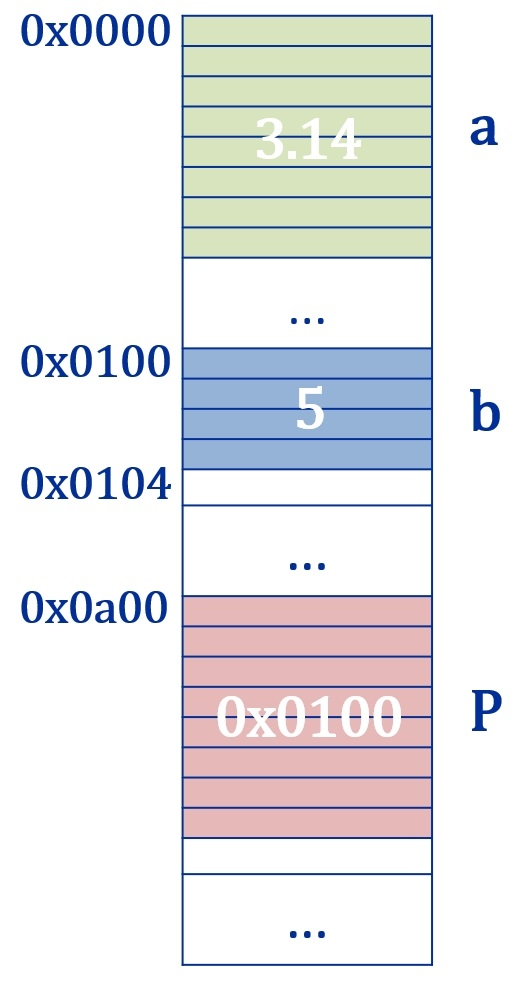
\includegraphics[width=.66\textwidth]{ch21/addressOfMemory.png}
        \end{figure}
    \end{columns}
\end{frame}
%------------------------------------------------------------

%------------------------------------------------------------
\begin{frame}[fragile]
    \frametitle{指针的声明}

    \begin{columns}
        \column{.65\textwidth}
        \begin{itemize}[<+->]
           \item 指针的声明需要添加一个星号,表示该变量为指针变量
            \begin{itemize}
               \item \lstinline|double *p;| 声明了一个名为 p 的指针变量,可用于储存 \lstinline|double| 类型变量的地址
               \item 如果 $p$ 储存了 $x$ 的地址,我们称\textbf{指针 $p$ 指向 $x$}
               \item 如果要储存 \lstinline|int| 类型变量的地址,如何声明指针?
            \end{itemize}
        \end{itemize}

        \column{.35\textwidth}
        \begin{figure}
            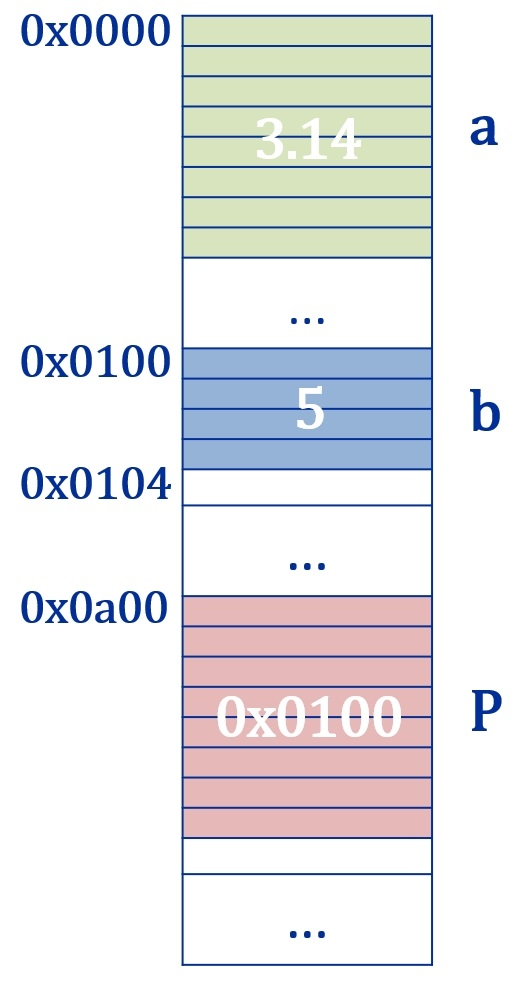
\includegraphics[width=.66\textwidth]{ch21/addressOfMemory.png}
        \end{figure}
    \end{columns}
\end{frame}
%------------------------------------------------------------

%------------------------------------------------------------
\begin{frame}[fragile]
    \frametitle{取地址和解引用运算符}

    \begin{itemize}
       \item \textbf{取地址运算符}:\lstinline|&x| 可以获得变量 $x$ 在内存中的地址
       \item \textbf{解引用运算符}:\lstinline|*p| 可以获得指针变量 $p$ 所指向的变量
    \end{itemize}

    \begin{columns}
        \column{.01\textwidth}

        \column{.25\textwidth}
        \lstinputlisting[basicstyle=\ttfamily\scriptsize,language=C++,name=pointer]{ch21/pointer.cc}
        \begin{tikzpicture}[remember picture,overlay]
            \only<1>{\redbox{pointer}{2}{1}{2}{13};}
            \only<2>{\redbox{pointer}{3}{1}{3}{13};}
            \only<3>{\redbox{pointer}{4}{1}{4}{13};}
            \only<4-5>{\redbox{pointer}{5}{1}{5}{13};}
        \end{tikzpicture}

        \column{.74\textwidth}
        \alt<3-5>{
            \alt<3>{
                \begin{tikzpicture}
                [nodes in empty cells, nodes={minimum width=1.3cm, minimum height=.7cm}, row sep=-\pgflinewidth, column sep=-\pgflinewidth]
                    \matrix(a) [matrix of nodes, ampersand replacement=\&, row 1/.style={nodes={draw=none}},row 3/.style={nodes={draw=none}}, column 1/.style={nodes={draw=none, font=\footnotesize}}, nodes={draw, anchor=center}]{
                        变量名   \& \lstinline| | \& \lstinline|x| \& \lstinline| | \& \lstinline|p| \& \lstinline| |  \\
                        变量的值 \& \lstinline|...| \& \lstinline|5| \& \lstinline| | \& \lstinline|0x0100| \& \lstinline|...| \\
                        内存地址 \& \lstinline|...| \& \lstinline|0x0100| \& \lstinline| | \& \lstinline|0x00f4| \& \lstinline| | \\
                    };
                \end{tikzpicture}
            }{
                \begin{tikzpicture}
                [nodes in empty cells, nodes={minimum width=1.3cm, minimum height=.7cm}, row sep=-\pgflinewidth, column sep=-\pgflinewidth]
                    \matrix(a) [matrix of nodes, ampersand replacement=\&, row 1/.style={nodes={draw=none}},row 3/.style={nodes={draw=none}}, column 1/.style={nodes={draw=none, font=\footnotesize}}, nodes={draw, anchor=center}]{
                        变量名   \& \lstinline| | \& \lstinline|x| \& \lstinline| | \& \lstinline|p| \& \lstinline| |  \\
                        变量的值 \& \lstinline|...| \& \lstinline|6| \& \lstinline| | \& \lstinline|0x0100| \& \lstinline|...| \\
                        内存地址 \& \lstinline|...| \& \lstinline|0x0100| \& \lstinline| | \& \lstinline|0x00f4| \& \lstinline| | \\
                    };
                \end{tikzpicture}
            }
        }{
            \alt<1>{
                \begin{tikzpicture}
                [nodes in empty cells, nodes={minimum width=1.3cm, minimum height=.7cm}, row sep=-\pgflinewidth, column sep=-\pgflinewidth]
                    \matrix(a) [matrix of nodes, ampersand replacement=\&, row 1/.style={nodes={draw=none}},row 3/.style={nodes={draw=none}}, column 1/.style={nodes={draw=none, font=\footnotesize}}, nodes={draw, anchor=center}]{
                        变量名   \& \lstinline| | \& \lstinline|x| \& \lstinline| | \& \lstinline| | \& \lstinline| |  \\
                        变量的值 \& \lstinline|...| \& \lstinline|5| \& \lstinline| | \& \lstinline| | \& \lstinline|...| \\
                        内存地址 \& \lstinline|...| \& \lstinline|0x0100| \& \lstinline| | \& \lstinline| | \& \lstinline| | \\
                    };
                \end{tikzpicture}
            }{
                \begin{tikzpicture}
                [nodes in empty cells, nodes={minimum width=1.3cm, minimum height=.7cm}, row sep=-\pgflinewidth, column sep=-\pgflinewidth]
                    \matrix(a) [matrix of nodes, ampersand replacement=\&, row 1/.style={nodes={draw=none}},row 3/.style={nodes={draw=none}}, column 1/.style={nodes={draw=none, font=\footnotesize}}, nodes={draw, anchor=center}]{
                        变量名   \& \lstinline| | \& \lstinline|x| \& \lstinline| | \& \lstinline|p| \& \lstinline| |  \\
                        变量的值 \& \lstinline|...| \& \lstinline|5| \& \lstinline| | \& \lstinline| | \& \lstinline|...| \\
                        内存地址 \& \lstinline|...| \& \lstinline|0x0100| \& \lstinline| | \& \lstinline|0x00f4| \& \lstinline| | \\
                    };
                \end{tikzpicture}
            }
        }
    \end{columns}

        \begin{itemize}
           \item<4-> $p$ 指向 $x$ ,\lstinline|*p| 解引用获取 $x$ ,\lstinline|(*p)++| 相当于 \lstinline|x++ |
           \item<5> 解引用的运算优先级较低,使用时需要注意!
        \end{itemize}

\end{frame}
%------------------------------------------------------------

%------------------------------------------------------------
\begin{frame}[fragile]
    \frametitle{指向结构体变量的指针}

    \begin{itemize}
        \item<1-> 若定义了结构体 \lstinline|Student| ,成员变量有姓名 $name$ 和 年龄 $age$,思考以下代码的含义:
        \lstinputlisting[basicstyle=\ttfamily\scriptsize,language=C++,name=structPointer]{ch21/structPointer.cc}
        
        \item<2-> 除了 \textbf{(*指针).成员名},还可以通过 \textbf{指针->成员名} 获取结构体的成员
        \begin{itemize}
            \item \lstinline|(*p).name = "xm"| 也可以写成 \lstinline|p->name = "xm"|
        \end{itemize}
    \end{itemize}
\end{frame}
%------------------------------------------------------------

%------------------------------------------------------------
\begin{frame}[fragile]
    \frametitle{利用指针交换两个变量的值}
    \alt<2>{
        \begin{itemize}
            \item 传递指针变量,实参需取地址
            \lstinputlisting[basicstyle=\ttfamily\scriptsize,language=C++,name=swap2]{ch21/swap2.cc}
        \end{itemize}
    }{
        \begin{itemize}
            \item 传递引用变量
            \lstinputlisting[basicstyle=\ttfamily\scriptsize,language=C++,name=swap1]{ch21/swap1.cc}
        \end{itemize}
    }
    
\end{frame}
%------------------------------------------------------------

%------------------------------------------------------------
\begin{frame}[fragile]
    \frametitle{小结}

    \begin{itemize}
        \item 指针变量用于储存内存地址,若指针 $p$ 储存了 $x$ 的地址,称 $p$ 指向 $x$

        \item 运算符
        \begin{itemize}
            \item 取地址:\lstinline|&x| 获取变量 $x$ 在内存中的地址
            \item 解引用:\lstinline|*p| 获取指针 $p$ 所指向的变量
        \end{itemize}

        \item 指针变量所占用的空间大小不由变量类型决定,由操作系统决定
        \begin{itemize}
            \item $64$ 位操作系统的地址为 $64$ 位,需要使用 $8$ 个字节存储
        \end{itemize}
    \end{itemize}
    
\end{frame}
%------------------------------------------------------------

%------------------------------------------------------------
\begin{frame}[fragile]
    \frametitle{注意要点}

    \begin{table}[!ht]
        \centering
        \renewcommand{\arraystretch}{1.5} % 设置垂直内边距为1.5倍默认行高
        \begin{tabular}{p{0.8cm}p{3cm}p{3.6cm}p{1.6cm}}
            \hline
            \textbf{符号} & \textbf{用于声明变量}  & \textbf{单目运算}  & \textbf{双目运算} \\ \hline
            \lstinline|*| & \lstinline|int *p| & \lstinline|*p| & \lstinline|a * b| \\ 
            \lstinline| | & 标志变量为一个指针变量 & 解引用:得到指针 $p$ 所指向地址上的内容 &  乘法符号 \\ \hline
            \lstinline|&| & \lstinline|int &a| & \lstinline|&a| & \lstinline|a & b| \\ 
            \lstinline| | & 标志变量为一个引用类型 & 取地址:得到变量 $a$ 的地址 & 位与符号\\ \hline
        \end{tabular} 
    \end{table}

\end{frame}
%------------------------------------------------------------

\section{指针与数组}

%------------------------------------------------------------
\begin{frame}[fragile]
    \frametitle{指针与整数做加法}

    \begin{itemize}
        \item 假设有 $2$ 个相邻的 \lstinline|int| 变量 $x$ 和 $y$ ,由于 \lstinline|int| 变量占 $4$ 字节,它们的地址会相差 $4$ ,如下图:

        \begin{itemize}
            \item<2> 如果指针 $p$ 指向 $x$,$p + 1$ 也是指针,而且指向下一个元素 $y$ ,不是指向下一个字节
        \end{itemize}
    \end{itemize}

    \alt<2>{
        \begin{tikzpicture}
        [nodes in empty cells, nodes={minimum width=1.3cm, minimum height=.7cm}, row sep=-\pgflinewidth, column sep=-\pgflinewidth]
            \matrix(a) [matrix of nodes, ampersand replacement=\&, row 1/.style={nodes={draw=none}}, row 3/.style={nodes={draw=none}}, row 4/.style={nodes={draw=none}}, column 1/.style={nodes={draw=none, font=\footnotesize}}, nodes={draw, anchor=center}]{
                变量名   \& \lstinline| | \& \lstinline|x| \& \lstinline|y| \&  \lstinline| |  \\
                变量的值 \& \lstinline|...| \& \lstinline|5| \& \lstinline|1| \&  \lstinline|...| \\
                内存地址 \& \lstinline|...| \& \lstinline|0x0100| \& \lstinline|0x0104| \& \lstinline|...| \\
                指针  \& \lstinline| | \& \lstinline|p| \& \lstinline|p+1| \&  \lstinline| |  \\
            };
        \end{tikzpicture}
    
    }{
        \begin{tikzpicture}
        [nodes in empty cells, nodes={minimum width=1.3cm, minimum height=.7cm}, row sep=-\pgflinewidth, column sep=-\pgflinewidth]
            \matrix(a) [matrix of nodes, ampersand replacement=\&, row 1/.style={nodes={draw=none}},row 3/.style={nodes={draw=none}}, column 1/.style={nodes={draw=none, font=\footnotesize}}, nodes={draw, anchor=center}]{
                变量名   \& \lstinline| | \& \lstinline|x| \& \lstinline|y| \&  \lstinline| |  \\
                变量的值 \& \lstinline|...| \& \lstinline|5| \& \lstinline|1| \&  \lstinline|...| \\
                内存地址 \& \lstinline|...| \& \lstinline|0x0100| \& \lstinline|0x0104| \& \lstinline|...| \\
            };
        \end{tikzpicture}
    }

\end{frame}
%------------------------------------------------------------

%------------------------------------------------------------
\begin{frame}[fragile]
    \frametitle{指针与指针做减法}

    \begin{itemize}
        \item 指针 $+$ 整数 $=$ 指针,那么 指针 $-$ 指针 $= ?$

        \begin{itemize}
            \item<2-> 指针 $-$ 指针 的结果是\textbf{整数类型},表示两个指针储存的地址之间相差的元素个数
            \item<3-> 如下图,指针 $p$ 指向 $x$,指针 $q$ 指向 $y$,此时 $q - p$ 的值是 $2$
        \end{itemize}
    \end{itemize}

    \uncover<3>{
        \begin{tikzpicture}
        [nodes in empty cells, nodes={minimum width=1.3cm, minimum height=.7cm}, row sep=-\pgflinewidth, column sep=-\pgflinewidth]
            \matrix(a) [matrix of nodes, ampersand replacement=\&, row 1/.style={nodes={draw=none}},row 3/.style={nodes={draw=none}},row 4/.style={nodes={draw=none}}, column 1/.style={nodes={draw=none, font=\footnotesize}}, nodes={draw, anchor=center}]{
                变量名   \& \lstinline| | \& \lstinline|x| \&  \lstinline| |  \& \lstinline|y| \&  \lstinline| |  \\
                变量的值 \& \lstinline|...| \& \lstinline|5| \&  \lstinline| | \& \lstinline|1| \&  \lstinline|...| \\
                内存地址 \& \lstinline|...| \& \lstinline|0x0100| \&  \lstinline|0x0104| \& \lstinline|0x0108| \& \lstinline|...| \\
                指针  \& \lstinline| | \& \lstinline|p| \& \&  \lstinline| | \lstinline|q| \&  \lstinline| |  \\
            };
        \end{tikzpicture}
    }

\end{frame}
%------------------------------------------------------------

%------------------------------------------------------------
\begin{frame}[fragile]
    \frametitle{指针与数组}

    \begin{itemize}
       \item<1-> 数组名在一定程度上可以看作是\textbf{指向数组首元素的指针常量}
       \item<1-> 声明数组 $a$:\lstinline|int a[10];|
            \begin{itemize}
                \item<1-> \lstinline|a == &a[0]|
                \item<2-> 根据指针与整数的加法规则:\lstinline|a + i == &a[i]|
                \item<3-> \lstinline|*(a + i) == a[i]|
                \item<4-> 注意常量不能修改,因此不能修改 $a$,比如 \lstinline|a += i| 会编译失败               
            \end{itemize}
    \end{itemize}
    
    \only<2>{
        \begin{tikzpicture}
        [nodes in empty cells, nodes={minimum width=1.3cm, minimum height=.7cm}, row sep=-\pgflinewidth, column sep=-\pgflinewidth]
            \matrix(a) [matrix of nodes, ampersand replacement=\&,row 2/.style={nodes={draw=none}}, column 1/.style={nodes={draw=none, font=\footnotesize}}, nodes={draw, anchor=center}]{
                变量   \& \lstinline|...| \& \lstinline|a[0]| \&  \lstinline|a[1]|  \& \lstinline|a[2]| \&  \lstinline|a[3]| \& \lstinline|...| \\
                内存地址 \& \lstinline|...| \& \lstinline|a| \&  \lstinline|a+1| \& \lstinline|a+2| \& \lstinline|a+3| \& \lstinline|...|\\
            };
        \end{tikzpicture}
    }

\end{frame}
%------------------------------------------------------------

%------------------------------------------------------------
\begin{frame}[fragile]
    \frametitle{函数参数传递数组}

    \begin{itemize}
       \item 数组名表示指向 $s[0]$ 的指针常量,本质上是传递指针
       \alt<2>{
            \lstinputlisting[basicstyle=\ttfamily\scriptsize,language=C++,name=functionParaArrayPointer]{ch21/functionParaArrayPointer.cc}
        }{
            \lstinputlisting[basicstyle=\ttfamily\scriptsize,language=C++,name=functionParaArray]{ch21/functionParaArray.cc}
        }
    \end{itemize}
    
\end{frame}
%------------------------------------------------------------

\section{C 语言的输入输出}

%------------------------------------------------------------
\begin{frame}[fragile]
    \frametitle{scanf 函数}

    \begin{itemize}
       \item \lstinline|scanf| 函数为 $C$ 语言的输入,其功能与 \lstinline|cin| 相似,但比 \lstinline|cin| 效率更高
       \item 调用语法是 \textbf{scanf(格式化字符串,变量地址列表)}
    
        \begin{itemize}
           \item<2-> 例如 \lstinline|scanf("%d", &a)| 表示读入数据到 \lstinline|int| 变量 $a$ 中,相当于 \lstinline|cin >> a|
           \item<2-> \lstinline|%d| 是格式说明符,表示读取十进制整数并按 \lstinline|int| 的编码方式储存
           \item<2-> \lstinline|&a| 表示将读取的数据从 \lstinline|&a| 这个地址开始储存,即赋值给 $a$
           \item<3> 拓展:读入两个整数的写法:\lstinline|scanf("%d%d", &a, &b)|
        \end{itemize}
    \end{itemize}
    
\end{frame}
%------------------------------------------------------------

%------------------------------------------------------------
\begin{frame}[fragile]
    \frametitle{printf 函数}

    \begin{itemize}
       \item \lstinline|printf| 函数为 $C$ 语言的输出,其功能与 \lstinline|cout| 相似,但比 \lstinline|cout| 效率更高
       \item 调用语法是 \textbf{printf(格式化字符串,变量列表)}
    
        \begin{itemize}
           \item<2-> 例如 \lstinline|printf("%d\n", a)| 表示输出变量 $a$ 并换行,相当于 \lstinline|cout << a << endl|
           \item<2-> \lstinline|%d| 是格式说明符,表示将变量 $a$ 的值按照十进制整数的形式输出
           \item<2-> \lstinline|\n| 是换行符
           \item<3> 拓展:\lstinline|printf("%d + %d\n", a, b)| 相当于 \lstinline|cout << a << " + " << b << endl;|
        \end{itemize}
    \end{itemize}
    
\end{frame}
%------------------------------------------------------------

%------------------------------------------------------------
\begin{frame}[fragile]
    \frametitle{常见的格式说明符}

    \begin{itemize}
       \item \lstinline|int:%d|
       \item \lstinline|long long:%lld|
       \item \lstinline|char:%c|
        \begin{itemize}
           \item \lstinline|scanf| 中 \lstinline|%c| 会读入空白字符,在 \lstinline|%c| 前面加空格可以跳过空白字符进行读取
        \end{itemize}
       \item \lstinline|double|:\lstinline|scanf| 中用 \lstinline|%lf| ,\lstinline|printf| 中用 \lstinline|%f|
       \item $C$ 风格字符串(\lstinline|char| 数组):\lstinline|%s|
    \end{itemize}
    
\end{frame}
%------------------------------------------------------------

%------------------------------------------------------------
\begin{frame}[fragile]
    \frametitle{控制格式输出}

    \begin{itemize}
       \item 控制场宽
        \begin{itemize}
           \item 在 \lstinline|%| 和字母中添加数字 $m$,指定输出的数据占据 $m$ 个字符的位置
        \end{itemize}
    \end{itemize}

   \begin{columns}
        \column{.01\textwidth}

        \column{.70\textwidth}
        \lstinputlisting[basicstyle=\ttfamily\scriptsize,language=C++,name=setwidth]{ch21/setwidth.cc}

        \column{.29\textwidth}
        \begin{itemize}
           \item 输出
            \begin{figure}
                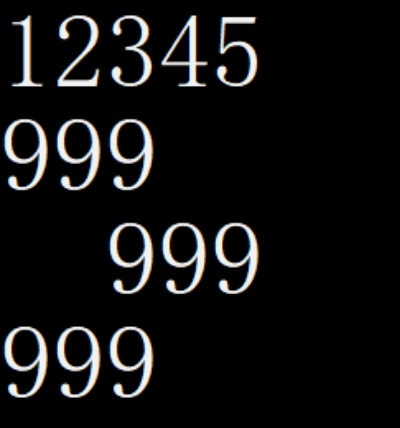
\includegraphics[width=.66\textwidth]{ch21/setwidth.png}
            \end{figure}
            
        \end{itemize}
   \end{columns}
    
\end{frame}
%------------------------------------------------------------

%------------------------------------------------------------
\begin{frame}[fragile]
    \frametitle{控制格式输出}

    \begin{itemize}
       \item 保留小数位
        \begin{itemize}
           \item 输出实数时,在 \lstinline|%| 和 \lstinline|f| 的中间加上 \lstinline|.X|,形如 \lstinline|%.Xf|,令实数以保留 $X$ 位小数的形式输出
        \end{itemize}
    \end{itemize}

   \begin{columns}
        \column{.01\textwidth}

        \column{.70\textwidth}
        \lstinputlisting[basicstyle=\ttfamily\scriptsize,language=C++,name=precision]{ch21/precision.cc}

        \column{.29\textwidth}
        \begin{itemize}
           \item 输出
            \begin{figure}
                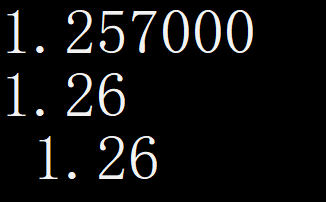
\includegraphics[width=.66\textwidth]{ch21/precision.png}
            \end{figure}
            
        \end{itemize}
   \end{columns}
    
\end{frame}
%------------------------------------------------------------

\section{总结}

%------------------------------------------------------------
\begin{frame}[fragile]
    \frametitle{内存空间与指针}

    \begin{itemize}
        \item<1-> 内存空间
            \begin{itemize}
                \item 栈空间、堆空间、全局区、代码段
            \end{itemize}
       \item<2-> 指针
            \begin{itemize}
                \item 储存内存地址
                \item 声明:\textbf{指向的元素类型 *指针名;}
                \item 取地址、解引用
                \item 指针的加减运算、与数组的联系
            \end{itemize}
       \item<3-> \lstinline|scanf| 和 \lstinline|printf| 函数的使用
    \end{itemize}
\end{frame}
%------------------------------------------------------------

%------------------------------------------------------------
\begin{frame}
    \begin{center}
        {\Huge Thank you!}
    \end{center}
\end{frame}
%------------------------------------------------------------

\end{document}
